\documentclass[12pt]{article}
\usepackage[margin=1.25in]{geometry}
\usepackage{amsmath,enumerate,graphicx,algorithm,algorithmic,caption,subcaption}

\begin{document}
\title{Counting jelly beans: voxel carving and segmentation of a container of heterogenous objects}
\author{Alex Cope, Mark O'Meara}
\date{March 2014}
\maketitle

\begin{abstract}

Foo

\end{abstract}

\section{Introduction}

\section{Prior Works}

I can talk about this: counting moving objects, generally.

\section{Approach}

\subsection{Voxel Carving}

\subsection{Segmentation}

We tried multiple approaches for solving the segmentation problem. The difficulty with using segmentation to count the number of objects in an image is that the algorithm must be robust to both false positives and false negatives; the count must be exact. The greater the number of objects in the scene, the more difficult this becomes. 

\subsubsection{Watershed}

We tried a couple classic blob detectors to count the number of beans and found limited success. The watershed algorithm, developed by Lindeberg (1993), detects blobs using local extrema in the image space \cite{Wshed}. We treat the grayscale image as a topographic surface, with lighter areas corresponding to maxima. Intuitively, we imagine flooding the topographic surface from its minima, and treat each resulting basin as a separate cluster. To reduce oversegmentation due to noise, we can flood the topographic surface from pre-defined markers. OpenCV contains an implementation of watershed but requires the markers to be passed in by the user; we wrote

\subsubsection{Mean-shift}

Intuitively, mean-shift seeks the modes of a feature space. That is, given a certain distribution in some feature space, mean-shift seeks the local maxima of the density of the distribution. Mean-shift associates a window around each data point, then computes the mean of the data within the window. It then shifts the window to its mean and repeats until the window location converges.

Mean

\section{Experiments}

\subsection{Segmentation}

\begin{figure}
    \centering
  \begin{subfigure}[b]{0.3\textwidth}
      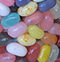
\includegraphics[width=\textwidth]{fig/img3}
      \caption{Unaltered.}
  \end{subfigure}
   \begin{subfigure}[b]{0.3\textwidth}
      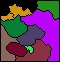
\includegraphics[width=\textwidth]{fig/wshed3}
      \caption{Watershed.}
  \end{subfigure}
   \begin{subfigure}[b]{0.3\textwidth}
      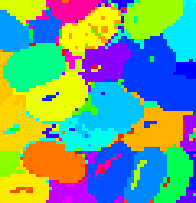
\includegraphics[width=\textwidth]{fig/ms3}
      \caption{Mean-shift.}
  \end{subfigure}
  \caption{Unaltered photo (a). Watershed (b) and mean shift (c) segmentation results. Different colors represent different clusters. (The black lines in the watershed picture are for clarity; they are omitted in the mean-shift picture due to the number of small clusters.)}
  \label{fig:unalt}
  \end{figure}

Different segmentation approaches were testing on the same small (60x60) cropped image of jellybeans (Fig.~\ref{fig:unalt}a). A cropped image was used to speed up runtime while iterating through refinements; this was necessary for mean-shift, which runs in \(O(n^2)\) and has two user defined parameters that drastically affect the final result.

Watershed (Fig.~\ref{fig:unalt}b) performs poorly compared to mean-shift; it is able to correctly identify one jellybean (in maroon) and otherwise grossly underestimates the number of clusters.

Mean-shift (Fig.~\ref{fig:unalt}c) performs much better. However, we can see from the image that it is susceptible to noise and texture (for example, see the number of small clusters it detects on the speckled jellybean at the top) and thus overestimates the number of clusters.

\begin{figure}
    \centering
  \begin{subfigure}[b]{0.3\textwidth}
      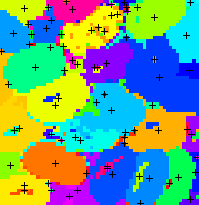
\includegraphics[width=\textwidth]{fig/ms_manyclusters}
      \caption{All clusters.}
  \end{subfigure}
   \begin{subfigure}[b]{0.3\textwidth}
      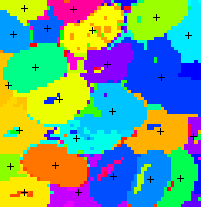
\includegraphics[width=\textwidth]{fig/ms_someclusters}
      \caption{Filtered clusters.}
  \end{subfigure}
   \begin{subfigure}[b]{0.3\textwidth}
      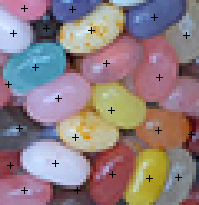
\includegraphics[width=\textwidth]{fig/ms_clustersoverimage}
      \caption{Over image.}
  \end{subfigure}
  \caption{Cluster centroids found using mean-shift.}
  \label{fig:clusters}
  \end{figure}

However, we can mitigate this overestimate by culling the clusters using a simple heuristic. We calculate the centroid, area, and variance of each cluster detected by the mean-shift algorithm. If the area is below and the variance above user-set thresholds, then the cluster is ignored. We see the results in Fig.~\ref{fig:clusters}. Fig.~\ref{fig:clusters}a shows all of the cluster centroids detected by mean-shift ($N = 78$), and Fig.~\ref{fig:clusters}b shows only the clusters with area $>$ 25 and variance $<$ 1000 ($N = 24$).  These threshold values are obviously affected by the scale of the image; however, because the noisy clusters are all small and all of the jellybeans are roughly the same size, the threshold values can be estimated roughly (i.e. they do not have to be fine-tuned for good performance.)

Quantitatively, we see that this cluster detection algorithm performs remarkably well (Fig.~\ref{fig:clusters}c). It is able to correctly count all but one jellybean on the front layer, and even correctly identifies some of the occluded jellybeans below the front layer.

One difficulty with mean-shift is that the two user-defined parameters ($h$ and histogram count) drastically affect the final cluster output. There is no automatic way to tune these; one must simply inspect and tune them based on the output. If $h$ is too small, the algorithm will be too sensitive and it will detect too many clusters; also, the algorithm will take much longer to converge. On the other hand, if $h$ is too large, the algorithm will incorrectly merge distinct clusters.

\begin{figure}
    \centering
  \begin{subfigure}[b]{0.3\textwidth}
      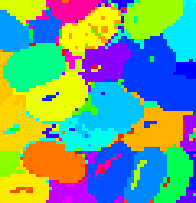
\includegraphics[width=\textwidth]{fig/ms3}
      \caption{$h=.8$}
  \end{subfigure}
   \begin{subfigure}[b]{0.3\textwidth}
      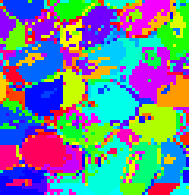
\includegraphics[width=\textwidth]{fig/h05}
      \caption{$h=.5$}
  \end{subfigure}
   \begin{subfigure}[b]{0.3\textwidth}
      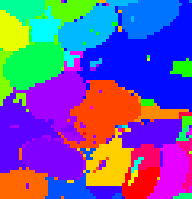
\includegraphics[width=\textwidth]{fig/h12}
      \caption{$h=1.2$}
  \end{subfigure}
  \caption{Mean-shift results using different values of $h$.}
  \label{fig:h}
  \end{figure}

We see this demonstrated in Fig.~\ref{fig:h}. Fig.~\ref{fig:h}a-c show the algorithm run with $h =$ 0.8, 0.5, and 1.2 respectively. We see that with low $h$, clusters are more susceptible to noise and more likely to bisect jellybeans. With high $h$, multiple jellybeans are more likely to be clustered together.

\section{Conclusion}

Ultimately, 

\begin{thebibliography}{9}

\bibitem{Wshed}
	Serge Beucher,
	\emph{Image segmentation and mathematical morphology.}
	http://cmm.ensmp.fr/~beucher/wtshed.html, May 2010.

\end{thebibliography}

\end{document}